\setcounter{section}{58}
\section{Sparse Table: модельная задача, построение за $O(n \log n)$, ответ на запрос за $O(1)$. }
\noindent Пусть даны \underline{неизменяемые} объекты $a_1, \ldots, a_n$ и задача найти минимум на отрезке $[l,r]$.
\\ \par \noindent \textbf{Разреженная таблица} — двумерная структура данных $ST[j][i]$, для которой выполнено следующее:
\begin{itemize}
    \item $\forall i \quad ST[0][i] = a_i$
    \item $ST[j+1][i]= min\{ST[j][i], ST[j][p]\}$, \quad где $p=min\{n,i+2^j\}$
\end{itemize}
Иначе говоря, в этой таблице хранятся минимумы на всех отрезках, длины которых равны степеням двойки. \textbf{Объём памяти}, занимаемый таблицей, равен $O(n\log n)$, и заполненными являются только те элементы, для которых $i+2j\leq n$.
\newline Такая простота достигается за счет идемпотентности операции минимум: $min(a,a)=a$. Это один из ключевых моментов этого метода, так как она позволяет нам корректно считать минимум в области пересечения отрезков.
\\ \par \textbf{Лемма: } Если $k=max\{k\;|\;2^k\leq r-l+1\}$, тогда отрезки $[l,l+2^k-1]$ и $[r-2^k+1, r]$ пересекаются.
\par \noindent $\blacktriangle$ Пусть отрезки не пересекаются, тогда $l+2^k-1 < r-2^k+1 \quad \Rightarrow \quad r-l+1\geq 2^k + 2^k$. Противоречие выбору $k$. \quad $\blacksquare$
\\ \par \noindent Поэтому \textbf{ответ на запрос минимума} на отрезке $[l,r]$ есть $min\{ST[k][l], ST[k][r-2^k+1]\}$. Чтобы ответ на запрос был за $O(1)$ необходимо предпосчитать $k$ для всех $len = 1, \ldots, n$.
Для этого введем функцию $fl$ (от floor, т.к. логарифм округляется вниз). Вычисление $fl[len]$ происходит за $O(\log len)$. А так как длина может принимать $n$ различных значений, то суммарное время предпосчета составляет $O(n\log n)$.
\begin{figure}[h]
    \hspace{-4ex} \begin{minipage}[h]{0.6\linewidth}
    \center{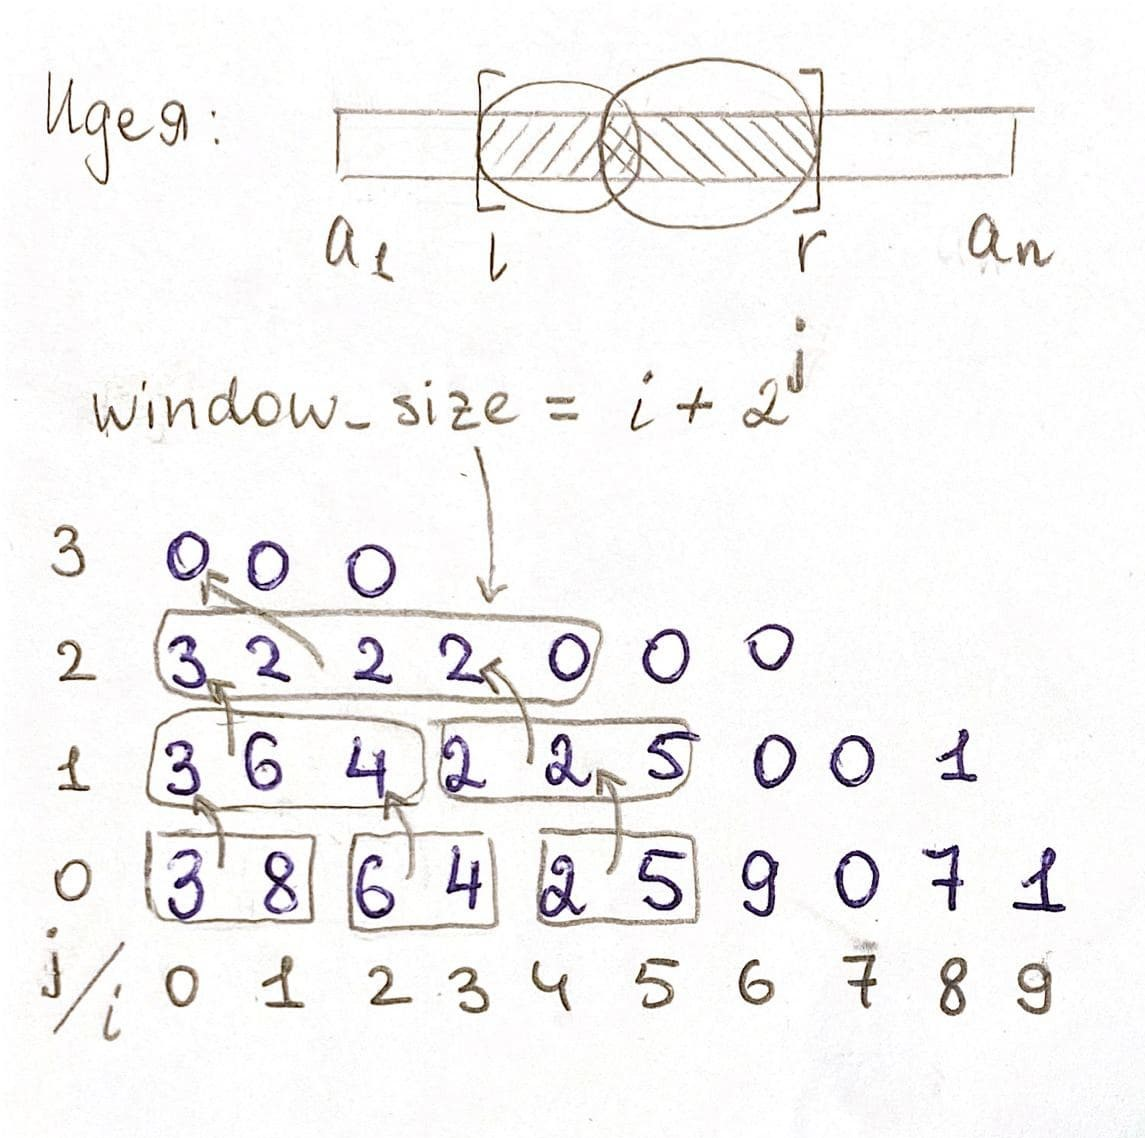
\includegraphics[width=0.8\linewidth]{images/59_1}}
    \end{minipage}
    \hfill
    \hspace{-4ex} \begin{minipage}[h]{0.5\linewidth}
    \center{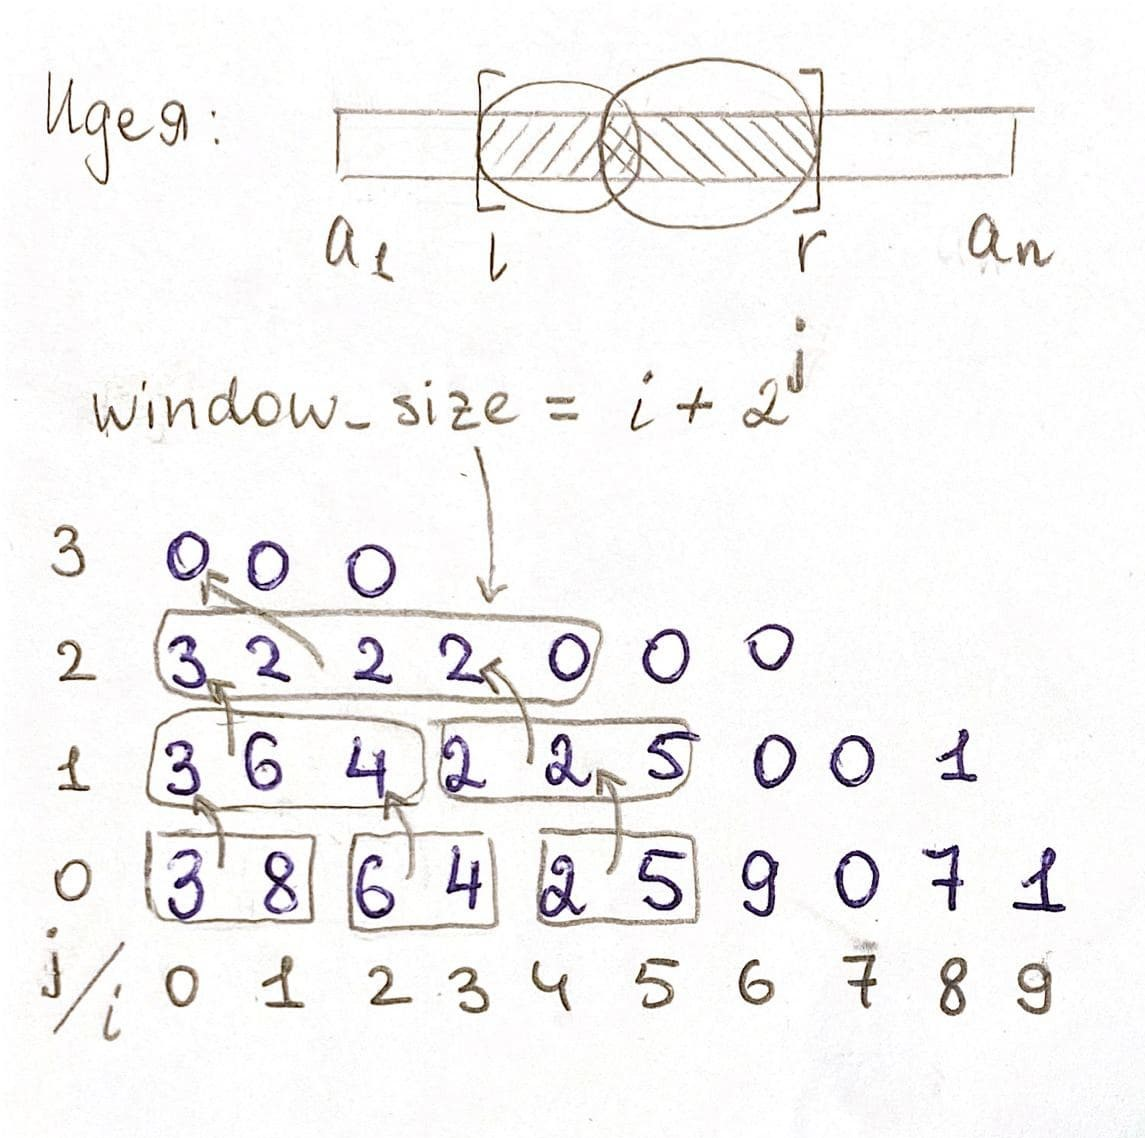
\includegraphics[width=0.8\linewidth]{images/59_1}}
    \end{minipage}
\end{figure}